\subsection{Problema 2}

\textit {“Un profesor tiene un salario inicial de \$1500, y percibe un incremento de 10\% anual durante 6 años. ¿Cuál es su salario al cabo de 6 años? ¿Qué salario ha recibido en cada uno de los 6 años?”}

\textbf{Modelo}

En el modelo se especifican 3 atributos para realizar los cálculos. Siendo estos:

\begin{center}
\begin{lstlisting}
final double salarioInicial;
final double incremento;
final int anios;
\end{lstlisting}
\end{center}

Así, se las incorporarían dentro de un método para calcular los salarios del profesor a través de 5 años (ya que el primer año es el salario inicial). Para ello se va armando una lista donde se multiplica por 0.10 el salario actual de la persona.

\begin{center}
\begin{lstlisting}
List<double> calcularSalarios() {
  List<double> salarios = [salarioInicial];
  double actual = salarioInicial;

  for (int i = 1; i <= anios; i++) {
    actual += actual * incremento;
    salarios.add(double.parse(actual.toStringAsFixed(2)));
  }

  return salarios;
}
\end{lstlisting}
\end{center}

Finalmente, se obtiene el salario final de la persona, al tomar el último elemento de la lista.

\begin{center}
\begin{lstlisting}
double obtenerSalarioFinal() {
  return calcularSalarios().last;
}
\end{lstlisting}
\end{center}

\textbf{Controlador}

El controlador hace uso del modelo anterior. En este caso, la función devuelve un \lstinline{Map$<>$} que tiene dos argumentos: la lista de salarios y el salario final.

\begin{center}
\begin{lstlisting}
Map<String, dynamic> calcularSalarios(String salarioStr){ ... }
\end{lstlisting}
\end{center}

Para ello, primero se trata de verificar que el valor \lstinline{String} suministrado pueda ser convertido a un número decimal, de no ser el caso se retorna un mensaje de error.

\begin{center}
\begin{lstlisting}
try {
  double salario = double.parse(salarioStr);
  ...
} catch (e) {
  return {
  'error': "Ingresa un número válido para el salario inicial."
  };
}
\end{lstlisting}
\end{center}

Luego se utiliza el modelo, definiendo el salario inicial y calculando los salarios, por lo que al final se retorna tanto la lista de salarios como el salario final.

\begin{center}
\begin{lstlisting}
  final modelo = SalarioModel(salarioInicial: salario);
  final lista = modelo.calcularSalarios();

  return {
    'salarios': lista,
    'salarioFinal': modelo.obtenerSalarioFinal(),
  };
\end{lstlisting}
\end{center}

\textbf{Vistas}

En la vista principal, se hace uso de 3 variables para manejar el estado: el controlador, un mensaje de eror y el campo de texto del input. Con estas 3 variables, se las usa en la función \lstinline{calcular()}. En donde se realizan validaciones previas antes de utilizal el método del controlador y pasar a la siguiente pantalla de resutlados, donde se le pasa el \lstinline{Map} como argumento.

\begin{center}
\begin{lstlisting}
void calcular() {
    setState(() {
      errorMessage = null;
    });

    final input = salarioCtrl.text.trim();

    if (input.isEmpty) {
      setState(() {
        errorMessage = "Por favor, ingresa un salario inicial.";
      });
      return;
    }

    final salario = double.tryParse(input);

    if (salario == null) {
      setState(() {
        errorMessage = "El salario debe ser un número válido (sin letras ni símbolos).";
      });
      return;
    }

    if (salario <= 0) {
      setState(() {
        errorMessage = "El salario debe ser mayor que cero.";
      });
      return;
    }

    final resultado = controller.calcularSalarios(salarioCtrl.text);
    Navigator.pushNamed(context, 'teacher/result', arguments: resultado);
  }
\end{lstlisting}
\end{center}

Luego, en la vista de resultados, se recuperan los argumentos de la siguiente manera:

\begin{center}
\begin{lstlisting}
final resultado = ModalRoute.of(context)!.settings.arguments as Map<String, dynamic>;

final List<double>? salarios = resultado['salarios'] as List<double>?;
final double? salarioFinal = resultado['salarioFinal'] as double?;
\end{lstlisting}
\end{center}

\textbf{Ejecución}

De esta manera se pudo cumplir con el ejercicio propuesto, donde se dan a los 6 años de salario del profesor con un incremento del 10\% anual mediante las siguientes pantallas:

\begin{figure}[H]
    \centering
    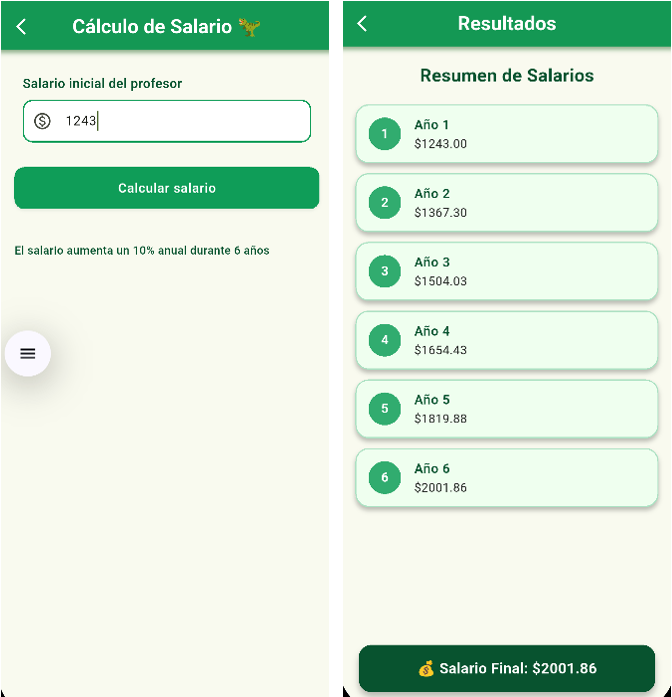
\includegraphics[width=0.8 \textwidth, height=8cm, keepaspectratio]{ejecucion_ej2.png}
    \caption{Ejecución ejercicio 2}
    \label{fig:ej2_ejecucion}
\end{figure}